\documentclass[aspectratio=169]{beamer}

\usepackage[utf8]{inputenc}
\usepackage[T1]{fontenc}
\usepackage[ngerman]{babel}
\usepackage{helvet}
\renewcommand{\familydefault}{\sfdefault}
\usepackage{graphicx}
\usepackage{amssymb} % \checkmark
\usepackage{tikz}
\usetikzlibrary{positioning, arrows.meta, calc, decorations.pathmorphing, patterns}

\graphicspath{{.}{../../sphinx/source/_images/individual_phase/}}

% ------------------------- Farbpalette -------------------------------
\definecolor{deepsea}{HTML}{0B1F33}   % dunkler Hintergrund
\definecolor{ocean}{HTML}{0E7C86}
\definecolor{teal}{HTML}{2EC4B6}      % Akzent
\definecolor{foam}{HTML}{E8F1F2}      % Text
\definecolor{coral}{HTML}{FF6B6B}     % Warnung / "naiv"
\definecolor{amber}{HTML}{F4A259}

% ------------------------- Look & Feel -------------------------------
\setbeamertemplate{navigation symbols}{}
\setbeamercolor{background canvas}{bg=deepsea}
\setbeamercolor{normal text}{fg=foam}
\setbeamercolor{frametitle}{fg=foam}
\setbeamercolor{structure}{fg=teal}
\setbeamercolor{itemize item}{fg=teal}

\setbeamerfont{frametitle}{size=\Large, series=\bfseries}

\setbeamertemplate{frametitle}{%
  \vspace*{0.55cm}%
  \hspace*{0.7cm}{\color{teal}\rule[-0.15ex]{3.5pt}{1.05em}}\hspace{0.45em}%
  \insertframetitle\par
}

\setbeamertemplate{footline}{%
  \hfill{\color{teal}\scriptsize \insertframenumber\,/\,\inserttotalframenumber}%
  \hspace{0.7cm}\vspace{0.35cm}%
}

\newcommand{\done}{{\color{teal}\bfseries \checkmark}}
\newcommand{\bonus}{{\color{amber}\bfseries +}}

% ---------------- Roter Faden: die Reise-Karte ------------------------
% 5 Stationen; pro Aufruf Stil je Station: ston (aktiv) / stoff (inaktiv)
\newcommand{\journeymap}[5]{%
  \begin{tikzpicture}[
      ston/.style={draw=teal, line width=1.4pt, rounded corners,
        fill=teal!35, text=black, font=\small\bfseries,
        minimum width=1.9cm, minimum height=0.85cm},
      stoff/.style={draw=foam!25, line width=1pt, rounded corners,
        fill=foam!10!deepsea, text=foam!45, font=\small,
        minimum width=1.9cm, minimum height=0.85cm},
      jpf/.style={-{Stealth}, foam!45, line width=1.1pt}]
    \node[#1] (s1) {Klick};
    \node[#2, right=0.7cm of s1] (s2) {Quelle};
    \node[#3, right=0.7cm of s2] (s3) {Welle};
    \node[#4, right=0.7cm of s3] (s4) {Bild};
    \node[#5, right=0.7cm of s4] (s5) {Live};
    \draw[jpf] (s1) -- (s2);
    \draw[jpf] (s2) -- (s3);
    \draw[jpf] (s3) -- (s4);
    \draw[jpf] (s4) -- (s5);
  \end{tikzpicture}}

% Trennfolie: Karte + Abschnittstitel + Sprecher
\newcommand{\divider}[7]{%
  \begin{frame}[plain]
    \centering
    \vspace{2.0cm}
    \journeymap{#1}{#2}{#3}{#4}{#5}
    \\[1.1cm]
    {\LARGE\bfseries #6}\\[0.4cm]
    {\color{foam!60}\small #7}
  \end{frame}}

% ------------------------- Metadaten ---------------------------------
\title{Echtzeit-Tsunamis}
\subtitle{Abschlusspräsentation --- Interaktive Visualisierung mit OpenGL}
\author{Mika Brückner, Yannik Köllmann, Jan Vogt}
\date{Juli 2026} % TODO: Vortragsdatum eintragen

% =====================================================================
\begin{document}

% ---------- Titel ------------------------------------------------------
\begin{frame}[plain]
  \centering
  \vspace{1.4cm}
  {\color{teal}\rule{2.2cm}{2.5pt}}\\[0.7cm]
  {\Huge\bfseries Echtzeit-Tsunamis}\\[0.45cm]
  {\large\color{foam!85} Abschlusspräsentation \quad\textbullet\quad Interaktive Visualisierung mit OpenGL}\\[1.4cm]
  {\color{foam!75}\small \insertauthor}\\[0.35cm]
  {\color{foam!55}\footnotesize Tsunami Lab \quad\textbullet\quad \insertdate}
\end{frame}

% ======================================================================
% JAN | Einleitung (~2,5 min)
% ======================================================================

% ---------- Das Versprechen -------------------------------------------
\begin{frame}{Das Versprechen vom 18.\ Juni}
  \vspace{0.8cm}
  \centering
  \begin{tikzpicture}[
      schritt/.style={draw=teal, line width=1pt, rounded corners,
        fill=ocean!25, text=black, align=center, font=\small,
        minimum width=2.5cm, minimum height=1.7cm},
      pfeil/.style={-{Stealth}, teal, line width=1.2pt}]
    \node[schritt] (a) {Gebiet\\wählen};
    \node[schritt, right=0.9cm of a] (b) {GEBCO lädt\\Bathymetrie};
    \node[schritt, right=0.9cm of b] (c) {Verwerfung +\\Stärke setzen};
    \node[schritt, right=0.9cm of c] (d) {Welle läuft\\\textbf{live}};
    \draw[pfeil] (a) -- (b);
    \draw[pfeil] (b) -- (c);
    \draw[pfeil] (c) -- (d);
  \end{tikzpicture}
  \\[1.1cm]
  {\large Kein Video. Keine Aufzeichnung.\\[0.15cm]
   Ein Klick. Der \textcolor{teal}{Ozean reagiert}.}
  \note{JAN, ~35s. Wiedererkennung: exakt die Grafik aus dem Pitch. Frage in
    den Raum: Haben wir geliefert? Antwort: naechste Folie.}
\end{frame}

% ---------- Geliefert ---------------------------------------------------
\begin{frame}{Geliefert}
  \vspace{0.3cm}
  \begin{columns}[T]
    \begin{column}{0.46\textwidth}
      \vspace{0.4cm}
      {\renewcommand{\arraystretch}{1.55}\large
      \begin{tabular}{@{}cl@{}}
        \done & Globus \& Regionswahl \\
        \done & GEBCO nativ (7{,}5\,GB) \\
        \done & 3D-Vorschau \\
        \done & Live-Simulation \\
        \done & Okada statt Gauß \\
        \done & 5 historische Szenarien \\
        \bonus & {\color{foam!75}\normalsize Tanioka--Satake, Solver 2--3$\times$} \\
      \end{tabular}}
    \end{column}
    \begin{column}{0.52\textwidth}
      \centering
      \vspace{0.15cm}
      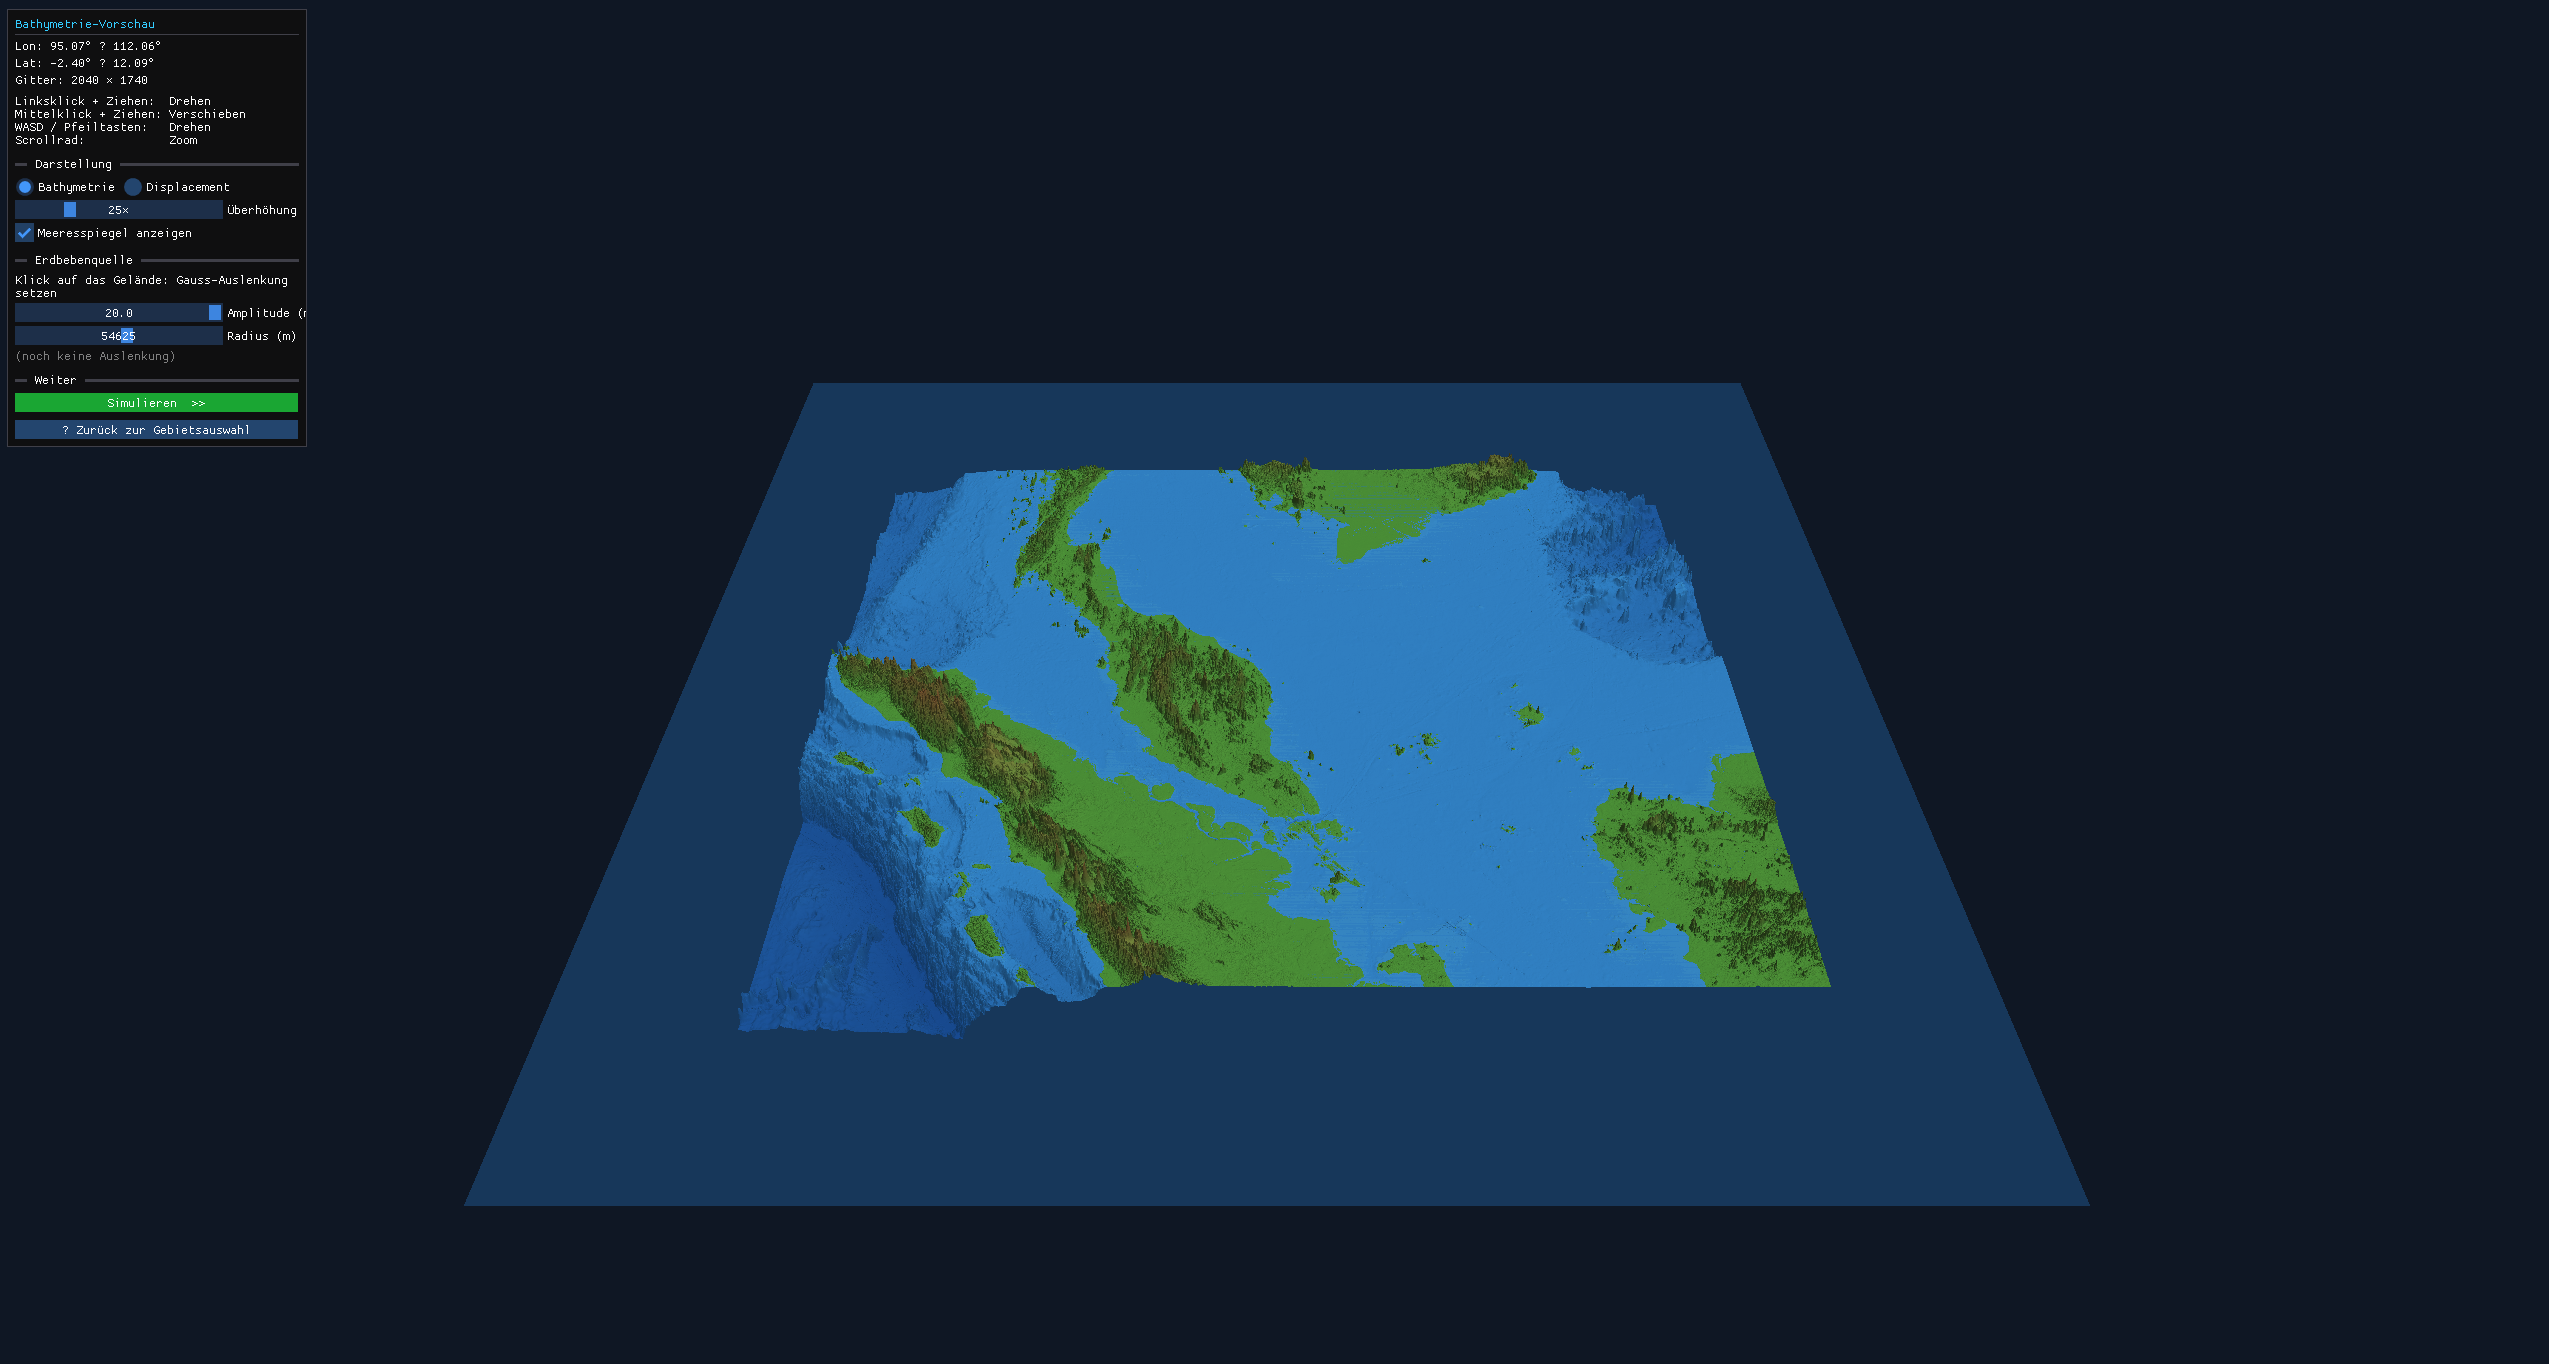
\includegraphics[width=\linewidth]{region_preview.png}\\[0.15cm]
      {\footnotesize\color{foam!70} GEBCO-Bathymetrie, live als 3D-Terrain}
    \end{column}
  \end{columns}
  \note{JAN, ~70s. Jede Zeile ist ein Pitch-Versprechen — kurz antippen,
    Details kommen in den Abschnitten. Letzte Zeile: Bonus, war nie
    versprochen. Ueberleitung: "Wie? Wir folgen einem Beben einmal durchs
    System."}
\end{frame}

% ---------- Der rote Faden ----------------------------------------------
\begin{frame}{Die Reise eines Bebens}
  \vspace{1.2cm}
  \centering
  \journeymap{ston}{ston}{ston}{ston}{ston}
  \\[1.0cm]
  {\large Ein Klick wird zur Verwerfung, die Verwerfung zur Welle,\\
   die Welle zum Bild --- \textcolor{teal}{in Echtzeit}.}\\[0.6cm]
  {\color{foam!60}\small Quelle: Mika \quad\textbullet\quad Welle \& Bild: Yannik \quad\textbullet\quad Live: alle}
  \note{JAN, ~30s. Die Karte ist der rote Faden — sie kommt vor jedem
    Abschnitt wieder. Uebergabe an Mika.}
\end{frame}

% ======================================================================
% MIKA | Klick -> Quelle (~4 min)
% ======================================================================
\divider{ston}{ston}{stoff}{stoff}{stoff}{Vom Klick zur Quelle}{Mika --- Okada-Modell \& Parameterbestimmung}

% ---------- 1 Zahl -> 9 Parameter --------------------------------------
\begin{frame}{Eine Magnitude $\rightarrow$ neun Parameter}
  \vspace{0.35cm}
  \centering
  \begin{tikzpicture}[
      quelle/.style={draw=teal, line width=1pt, rounded corners,
        fill=ocean!25, text=black, align=center, font=\footnotesize,
        minimum width=3.4cm, minimum height=1.2cm},
      annahme/.style={draw=foam!45, line width=1pt, rounded corners,
        fill=foam!12, text=black, align=center, font=\footnotesize,
        minimum width=3.4cm, minimum height=1.2cm},
      ziel/.style={draw=amber, line width=1.2pt, rounded corners,
        fill=amber!25, text=black, align=center, font=\small,
        minimum width=3.3cm, minimum height=2.2cm},
      pfeil/.style={-{Stealth}, teal, line width=1.2pt}]
    \node[quelle] (user) {\textbf{Nutzer}\\Klick + Magnitude $M_w$};
    \node[quelle, below=0.32cm of user] (slab) {\textbf{Slab2} (USGS)\\Tiefe, Streichen, Einfallen};
    \node[quelle, below=0.32cm of slab] (skal) {\textbf{Strasser 2010}\\Länge, Breite, Versatz};
    \node[annahme, below=0.32cm of skal] (fest) {\textbf{Feste Annahmen}\\Rake $90^\circ$, $\nu = 0{,}25$};
    \node[ziel, right=2.4cm of slab.east, yshift=-0.8cm] (okada)
      {\textbf{Okada}\\1985 / 1992\\[0.15cm]\footnotesize Verformung des\\Meeresbodens};
    \draw[pfeil] (user.east) -- (okada.west|-user.east) -- (okada);
    \draw[pfeil] (slab.east) -- (okada);
    \draw[pfeil] (skal.east) -- (okada);
    \draw[pfeil] (fest.east) -- (okada.west|-fest.east) -- (okada);
  \end{tikzpicture}
  \\[0.35cm]
  {\small Slab2 ist zugleich \textcolor{teal}{Plausibilitätsfilter} ---
   außerhalb von Subduktionszonen: Fallback Wells \& Coppersmith 1994.}
  \note{MIKA, ~80s. Sprechtext Abschnitte 1, 3, 4: eine Zahl vom Nutzer,
    neun fuer Okada — wer liefert was und warum. Rake und Poisson-Zahl
    betonen: bewusste Modellannahmen, keine Daten.}
\end{frame}

% ---------- Okada-Feld ---------------------------------------------------
\begin{frame}{Was der Meeresboden tut}
  \vspace{0.2cm}
  \centering
  \begin{tikzpicture}[scale=1.05]
    \useasboundingbox (-0.4,-0.3) rectangle (11.6,4.9);
    % Wasser
    \fill[ocean!25] (0,2.2) rectangle (11.2,3.9);
    % Meeresboden: verformt — Hebung ueber dem oberen Faultende, Senkung dahinter
    \draw[foam, very thick]
      (0,2.2) -- (2.6,2.2)
      .. controls (3.6,2.2) and (3.4,2.95) .. (4.4,2.95)
      .. controls (5.4,2.95) and (5.2,1.75) .. (6.6,1.75)
      .. controls (7.6,1.75) and (7.6,2.2) .. (8.6,2.2) -- (11.2,2.2);
    % Hebungs-/Senkungsflaechen
    \fill[amber!55, opacity=0.75]
      (2.6,2.2) .. controls (3.6,2.2) and (3.4,2.95) .. (4.4,2.95)
      .. controls (5.0,2.95) and (5.05,2.5) .. (5.35,2.2) -- cycle;
    \fill[ocean!70, opacity=0.9]
      (5.35,2.2) .. controls (5.6,1.85) and (5.9,1.75) .. (6.6,1.75)
      .. controls (7.6,1.75) and (7.6,2.2) .. (8.6,2.2) -- cycle;
    \node[black, font=\footnotesize\bfseries] at (4.1,2.55) {Hebung};
    \node[foam, font=\footnotesize\bfseries] at (6.9,2.0) {Senkung};
    % Wasseroberflaeche: folgt der Bodenverformung (gestrichelt, abgeschwaecht)
    \draw[teal, very thick, dashed]
      (0,3.9) -- (2.6,3.9)
      .. controls (3.5,3.9) and (3.5,4.25) .. (4.3,4.25)
      .. controls (5.1,4.25) and (5.2,3.62) .. (6.6,3.62)
      .. controls (7.6,3.62) and (7.7,3.9) .. (8.6,3.9) -- (11.2,3.9);
    \draw[-{Stealth}, teal, very thick] (4.3,3.92) -- (4.3,4.20);
    \draw[-{Stealth}, teal, very thick] (6.6,3.88) -- (6.6,3.66);
    \node[teal, font=\footnotesize, anchor=west] at (0.15,4.5)
      {Wasser folgt instantan};
    \node[foam!75, font=\footnotesize, anchor=east] at (11.1,4.12) {Meeresspiegel};
    % Verwerfung: Slip-Halbpfeile parallel zur Flaeche, beidseitig
    \draw[coral, line width=2pt] (3.2,1.9) -- (6.2,0.5);
    \draw[-{Stealth}, coral, thick] (5.3,1.18) -- (4.5,1.55);
    \draw[-{Stealth}, coral, thick] (4.3,1.15) -- (5.1,0.78);
    \node[coral, font=\footnotesize, align=left, anchor=west] at (6.7,0.9)
      {Verwerfung, Versatz $U$\\[-2pt]{\color{foam!70}(9 Parameter)}};
  \end{tikzpicture}
  \\[0.3cm]
  {\small\color{foam!85} Geschlossene Formel, keine FEM ---
   \textcolor{teal}{konstante Zeit pro Gitterzelle}.}\\[0.15cm]
  {\small validiert gegen \texttt{okada85.m} (IPGP):
   \textbf{81 Fälle}, max.\ Abweichung $\sim 5\cdot10^{-11}$}
  \note{MIKA, ~60s. Sprechtext Abschnitte 2 und 5: Okada = analytische
    Loesung fuer den elastischen Halbraum; deshalb interaktiv machbar.
    Validierung: Referenz unveraendert uebernommen, in Octave ausgewertet,
    zeilenweise verglichen — Fliesskomma-Rauschen.}
\end{frame}

% ---------- Tanioka & Satake --------------------------------------------
\begin{frame}{Der Trench-Effekt (Tanioka \& Satake 1996)}
  \vspace{0.2cm}
  \centering
  \begin{tikzpicture}[scale=1.0]
    \useasboundingbox (-0.3,-0.2) rectangle (11.4,3.7);
    % Wasser
    \fill[ocean!25] (0,0.2) rectangle (11.0,3.4);
    % Meeresboden: steile Flanke, rechts Plateau
    \fill[foam!60] (0,0.2) -- (11.0,0.2) -- (11.0,2.6) -- (7.0,2.6) -- (4.0,1.0) -- (0,1.0) -- cycle;
    \draw[foam, very thick] (0,1.0) -- (4.0,1.0) -- (7.0,2.6) -- (11.0,2.6);
    % Boden nach der Verschiebung: Flanke um u_x nach links gerueckt
    \draw[black!60, dashed, thick] (3.3,1.0) -- (6.3,2.6);
    % horizontale Verschiebung: Pfeil im Plateau
    \draw[-{Stealth}, amber, line width=2pt] (8.8,2.15) -- (7.6,2.15);
    \node[black!75, font=\footnotesize] at (8.6,1.75)
      {Boden schiebt sich seitlich: {\color{amber}$u_x$}};
    % fester Punkt auf der Flanke: Boden steigt
    \draw[-{Stealth}, teal, line width=2pt] (5.5,1.83) -- (5.5,2.62);
    \node[teal, font=\small\bfseries, anchor=west] at (5.75,3.0) {wirkt wie Hebung};
    % Erklaerung links ueber dem tiefen Wasser
    \node[black!75, font=\footnotesize, align=center] at (2.5,2.6)
      {an steiler Flanke schiebt sich\\höherer Boden unter denselben Punkt};
  \end{tikzpicture}
  \\[0.25cm]
  {\large $u_z^{\text{eff}} = u_z - \bigl(u_x\,\tfrac{\partial b}{\partial x}
    + u_y\,\tfrac{\partial b}{\partial y}\bigr)$}\\[0.25cm]
  {\small Tohoku \& Chile liegen direkt an einer Tiefseerinne ---
   deshalb eingebaut, in \textcolor{teal}{Vorschau und Live-Simulation}.}
  \note{MIKA, ~45s. Sprechtext Abschnitt 6. Bild traegt die Erklaerung;
    Formel nur nennen, nicht herleiten. Effektgroesse: bis zu mehrere zehn
    Prozent (Java 1994: ca.\ 43\,\%).}
\end{frame}

% ---------- Grenzen ------------------------------------------------------
\begin{frame}{Ehrlich eingeordnet}
  \vspace{0.5cm}
  \centering
  {\large Seit 1900: nur \textbf{fünf} Beben mit $M_w \ge 9$ ---\\
   dort kann kein Skalierungsgesetz präzise sein.}\\[0.7cm]
  \begin{columns}[T]
    \begin{column}{0.44\textwidth}
      \centering
      {\color{teal}\Large\checkmark}\\[0.2cm]
      {\color{teal}\textbf{Gut für}}\\[0.25cm]
      {\small Ankunftszeit\\[0.1cm] Größenordnung der Welle\\[0.1cm]
       Orientierung \& Lage der Quelle}
    \end{column}
    \begin{column}{0.44\textwidth}
      \centering
      {\color{coral}\Large$\times$}\\[0.2cm]
      {\color{coral}\textbf{Nicht für}}\\[0.25cm]
      {\small exakte Pegel an einer Station\\[0.1cm] reale Slip-Verteilung\\[0.1cm]
       geschichtete Erdkruste}
    \end{column}
  \end{columns}
  \note{MIKA, ~45s. Sprechtext Abschnitt 7. Die Fuenf-Beben-Zahl ist das
    Kernargument (Kamtschatka 52, Chile 60, Alaska 64, Sumatra 04, Tohoku 11).
    Tohoku gilt zudem als Ausreisser — Details im Q\&A.}
\end{frame}

% ======================================================================
% YANNIK | Quelle -> Welle -> Bild (~4,5 min)
% ======================================================================
\divider{stoff}{stoff}{ston}{ston}{stoff}{Von der Quelle aufs Display}{Yannik --- Live-Simulation \& Performance}

% ---------- Threads ------------------------------------------------------
\begin{frame}{Drei Arten von Threads, ein Ozean}
  \vspace{0.5cm}
  \centering
  \begin{tikzpicture}[
      block/.style={draw=teal, line width=1.2pt, rounded corners,
        fill=ocean!25, text=black, align=center, font=\normalsize,
        minimum width=3.6cm, minimum height=1.8cm},
      buf/.style={draw=amber, line width=1.2pt, rounded corners,
        fill=amber!25, text=black, align=center, font=\normalsize,
        minimum width=3.0cm, minimum height=1.8cm},
      pfeil/.style={-{Stealth}, teal, line width=1.6pt}]
    \node[block] (gui) {GUI / Render\\{\footnotesize 60 FPS}};
    \node[buf, right=1.7cm of gui] (buf) {SimBuffer\\{\footnotesize Doppelpuffer}};
    \node[block, right=1.7cm of buf] (solver) {SolverThread\\{\footnotesize CFL $\rightarrow$ timeStep}};
    \node[block, below=0.7cm of solver, minimum height=1.1cm]
      (omp) {OpenMP-Pool {\footnotesize(P-Cores)}};
    \draw[pfeil] (buf) -- node[above, midway, foam!85, font=\small]{front} (gui);
    \draw[pfeil] (solver) -- node[above, midway, foam!85, font=\small]{back} (buf);
    \draw[pfeil, transform canvas={xshift=-2.5mm}] (solver) -- (omp);
    \draw[pfeil, transform canvas={xshift=2.5mm}] (omp) -- (solver);
    \node[coral, font=\small, align=center] at (2.9,-1.95)
      {\texttt{try\_lock}: im Konfliktfall fliegt der Frame weg ---\\
       \textbf{nie} der Solver in die Warteschleife};
  \end{tikzpicture}
  \\[0.5cm]
  {\large Der Renderer sieht immer den \textcolor{teal}{neuesten fertigen} Frame.}
  \note{YANNIK, ~70s. Kernidee Entkopplung: Renderer und Solver takten
    unabhaengig. Verlorene Frames egal (nur der neueste Zustand zaehlt).
    GUI-Thread ist der einzige ohne OpenMP — deshalb explizit gepinnt
    (TSUNAMI\_VIZ\_CORE). dt kommt pro Schritt frisch aus der CFL-Bedingung.}
\end{frame}

% ---------- Warum live geht: kein Datei-IO ------------------------------
\begin{frame}{Früher: rechnen, schreiben, warten}
  \vspace{0.3cm}
  \centering
  {\small Gleiche Simulation, $10^6$ Zellen, 793 Zeitschritte, 10 Threads (M4) ---
   Gesamtlaufzeit:}\\[0.5cm]
  \begin{tikzpicture}[yscale=0.86]
    % Balken: 0.96 s / 1.10 s / 8.9 s  -> Breite = s * 1.15 cm
    \fill[teal!80]  (0,2.4) rectangle (1.10,2.9);
    \fill[foam!45]  (0,1.4) rectangle (1.27,1.9);
    \fill[coral!85] (0,0.0) rectangle (10.2,0.5);
    \node[foam, anchor=west, font=\small\bfseries] at (1.3,2.65) {0{,}96 s};
    \node[foam, anchor=west, font=\small\bfseries] at (1.5,1.65) {1{,}1 s};
    \node[black, anchor=east, font=\small\bfseries] at (10.05,0.25) {8{,}9 s};
    \node[foam, anchor=west, font=\small] at (0.1,3.30)
      {\textbf{Live-Pfad} --- Frames in den Puffer, keine Dateien};
    \node[foam, anchor=west, font=\small] at (0.1,2.10)
      {NetCDF-Snapshots alle 25 Schritte \quad {\color{foam!60}371 MB}};
    \node[foam, anchor=west, font=\small] at (0.1,0.70)
      {NetCDF \textbf{jeden} Schritt (= „live'` über Dateien) \quad {\color{coral}8{,}9 GB}};
  \end{tikzpicture}
  \\[0.5cm]
  {\large Live über Dateien wäre $\sim$\textcolor{coral}{9$\times$ langsamer} ---
   $\sim$90\,\% der Zeit wäre Schreiben.}
  \note{YANNIK, ~55s. Der alte Workflow: rechnen, NetCDF schreiben, in
    ParaView laden, ansehen. Der Viz-Pfad kopiert pro Schritt 4 MB in den
    RAM-Puffer statt 12 MB synchron auf die Platte. Messung: 3 Runden
    verschraenkt, DamBreak2d 1000x1000, --io-steps 0/25/1.}
\end{frame}

% ---------- Parallelisierung: Kern-Aufteilung ---------------------------
\begin{frame}{Ein Kern zeigt, die anderen rechnen}
  \vspace{0.5cm}
  \centering
  \begin{tikzpicture}
    % CPU-Gehaeuse
    \draw[foam!40, line width=1.2pt, rounded corners] (-0.3,-1.6) rectangle (11.5,3.0);
    \node[foam!50, font=\footnotesize, anchor=north west] at (-0.1,2.9) {CPU};
    % Kern 0: Visualisierung & Datenaustausch
    \draw[amber, line width=1.4pt, rounded corners, fill=amber!25]
      (0.2,0.2) rectangle (2.9,2.4);
    \node[black, font=\small\bfseries, align=center] at (1.55,1.5)
      {Visualisierung \&\\Datenaustausch};
    \node[black!70, font=\footnotesize] at (1.55,0.6) {GUI-Thread};
    % Performance-Kerne: Solver
    \foreach \i in {0,1,2}{
      \draw[teal, line width=1.4pt, rounded corners, fill=ocean!30]
        ({3.4+\i*2.75},0.2) rectangle ({5.85+\i*2.75},2.4);
      \node[black, font=\small\bfseries] at ({4.62+\i*2.75},1.5) {Solver};
      \node[black!70, font=\footnotesize] at ({4.62+\i*2.75},0.6) {OpenMP};
    }
    % Beschriftung unten
    \node[amber, font=\footnotesize, align=center] at (1.55,-0.85)
      {\textbf{1 Kern}, fest gepinnt ---\\Bild bleibt flüssig};
    \node[teal, font=\footnotesize, align=center] at (7.4,-0.85)
      {\textbf{die übrigen Performance-Kerne} ---\\ein Solver-Thread pro Kern, ungestört};
  \end{tikzpicture}
  \\[0.6cm]
  {\large Solver und Bild kommen sich \textcolor{teal}{nie in die Quere}.}
  \note{YANNIK, ~40s. Nur die Aufteilung erzaehlen: ein Kern fuer GUI und
    Datenaustausch (fest gepinnt, TSUNAMI\_VIZ\_CORE), die uebrigen
    Performance-Kerne rechnen den Solver (OpenMP, ein Thread pro Kern).
    Speedup-Zahlen bewusst nicht auf der Folie — stehen im Q\&A, falls
    jemand fragt.}
\end{frame}

% ---------- CFL-Story ----------------------------------------------------
\begin{frame}{Als die Welle die Küste erreichte}
  \vspace{0.3cm}
  \begin{columns}[T]
    \begin{column}{0.47\textwidth}
      \vspace{0.3cm}
      {\color{coral}\textbf{Symptom}}\\[0.05cm]
      {\small Zeitraffer $\to$ 0 bei Landkontakt ---\\
       CPU, GPU, RAM: unauffällig.}\\[0.45cm]
      {\color{amber}\textbf{Diagnose}}\\[0.05cm]
      {\small cm-dünne Zellen am Nass/Trocken-Front:\\
       $u \approx 17\,000$ m/s $\Rightarrow$ CFL-dt $\div\,86$.}\\[0.45cm]
      {\color{teal}\textbf{Fix}}\\[0.05cm]
      {\small Froude-Limiter $|u| \le 2\sqrt{g\,h}$ ---\\
       echte Auflauffronten bleiben unberührt.}
    \end{column}
    \begin{column}{0.51\textwidth}
      \centering
      \vspace{0.1cm}
      \begin{tikzpicture}[scale=1.0]
        \useasboundingbox (-0.3,-0.75) rectangle (5.4,3.6);
        % Land
        \fill[foam!15] (0,0) -- (5.2,0) -- (5.2,2.1) -- (3.6,1.5) -- (2.1,0.6) -- (0,0.5) -- cycle;
        % Bore
        \fill[ocean!60] (0,0.5) -- (2.1,0.6) .. controls (2.5,0.65) and (2.55,2.3) .. (2.85,2.3) -- (0,2.3) -- cycle;
        \draw[-{Stealth}, foam, very thick] (0.6,1.6) -- (1.9,1.6);
        \node[foam, font=\footnotesize\bfseries] at (1.25,1.98) {Bore, 7 m};
        % duenner Film: liegt AUF dem Hang (Hangflaeche (2.1,0.6)-(3.6,1.5))
        \draw[coral, line width=2.2pt] (2.60,0.98) -- (3.35,1.43);
        \draw[-{Stealth}, coral] (3.75,2.72) -- (3.08,1.48);
        \node[coral, font=\footnotesize, align=center] at (3.9,3.15)
          {1 cm Wasserfilm\\$u \to 17\,000$ m/s};
        \node[foam!65, font=\footnotesize, align=center] at (2.6,-0.45)
          {dt kollabiert für das \textbf{gesamte} Gitter};
      \end{tikzpicture}
    \end{column}
  \end{columns}
  \note{YANNIK, ~60s. Story erzaehlen: Overlay faellt auf 0, alle Ressourcen
    normal — es kollabierte der Zeitschritt, nicht die Rechenleistung.
    Froude-Cap: Ritter-Front hat exakt Fr=2, gekappt wird nur der numerische
    Runaway (Fr~5000). Reproduziert im Testtreiber, Regressionstests.
    Falls gefragt: Reflexion an der Kueste explizit nachgemessen — Amplitude
    verdoppelt sich an der Wand (1,2 m), Land bleibt trocken (Details Q\&A).}
\end{frame}

% ======================================================================
% ALLE | Live (~4 min)
% ======================================================================

% ---------- Demo ---------------------------------------------------------
\begin{frame}[plain]
  \centering
  \vspace{1.5cm}
  \journeymap{stoff}{stoff}{stoff}{stoff}{ston}
  \\[0.9cm]
  {\LARGE\bfseries Der Ozean reagiert --- jetzt.}\\[0.8cm]
  {\color{foam!70}\small Tohoku laden \; $\rightarrow$ \; Okada-Feld prüfen \;
   $\rightarrow$ \; Simulation live \; $\rightarrow$ \; freier Klick}
  \note{ALLE, ~4 min. (1) Tohoku-Szenario laden, Okada-Feld zeigen — Mika
    kommentiert Hebung/Senkung und Slab2. (2) Simulation starten — Yannik
    kommentiert Zeitraffer, Kuestenaufprall, Reflexion. (3) Freier Klick +
    Klick ausserhalb der Subduktionszone (Slab2-Filter). Backup-Video
    vorher aufnehmen!}
\end{frame}

% ---------- Abschluss ----------------------------------------------------
\begin{frame}[plain]
  \centering
  \vspace{2.2cm}
  {\LARGE\bfseries Kein Video. Keine Aufzeichnung.\\[0.25cm]
   Ein Klick. Der \textcolor{teal}{Ozean reagiert}.}\\[1.2cm]
  {\color{foam!75} Versprochen am 18.\ Juni --- gezeigt heute.}\\[1.6cm]
  {\color{foam!55}\small Fragen?}
  \note{Moderation, ~15s. Callback auf die Pitch-Schlussfolie, Fragerunde.}
\end{frame}

\end{document}
